\documentclass[border=2pt]{standalone}
\usepackage[T1]{fontenc}
\usepackage{tikz}
\usetikzlibrary{arrows.meta, positioning, fit, backgrounds, calc, shapes.geometric}

\definecolor{setupfill}{HTML}{F1EFE8}
\definecolor{setupborder}{HTML}{5F5E5A}
\definecolor{loopfill}{HTML}{E1F5EE}
\definecolor{loopborder}{HTML}{0F6E56}
\definecolor{looptext}{HTML}{085041}
\definecolor{policyfill}{HTML}{EEEDED}
\definecolor{policyborder}{HTML}{534AB7}
\definecolor{policytext}{HTML}{3C3489}
\definecolor{arrowgray}{HTML}{737268}

\begin{document}
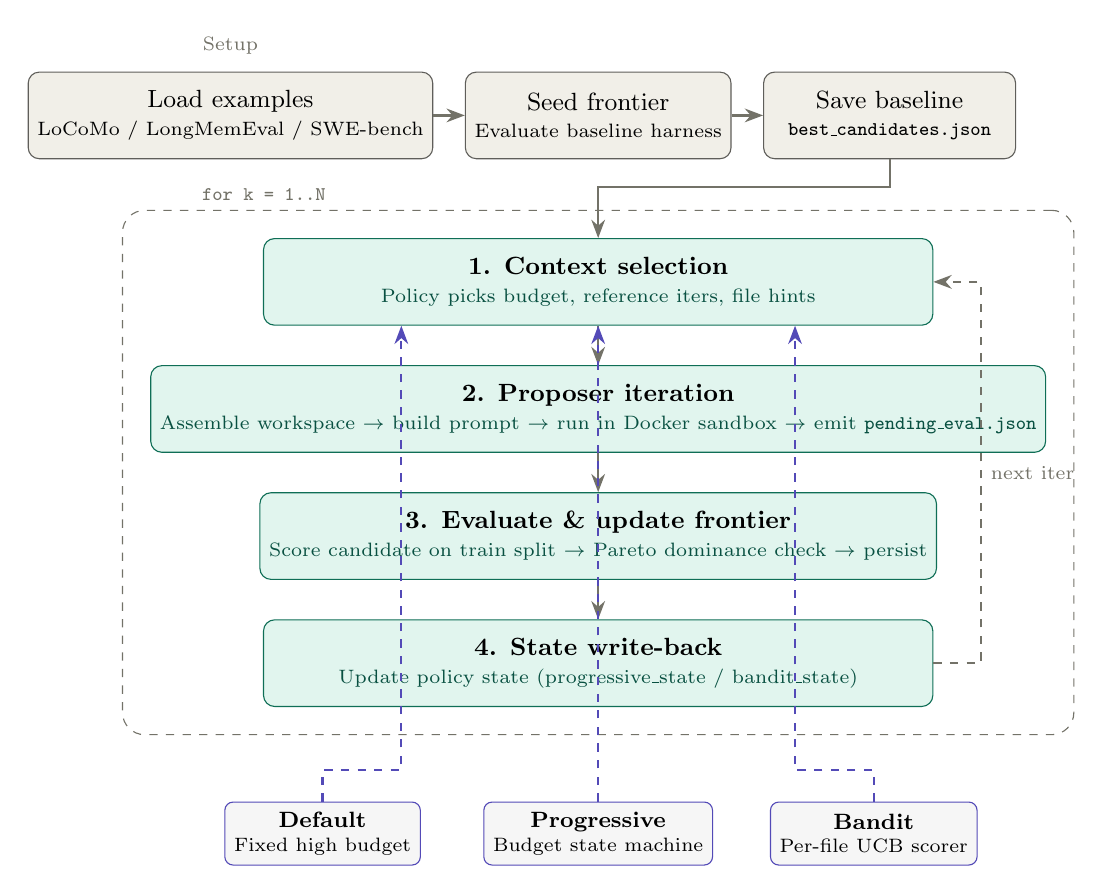
\begin{tikzpicture}[
    >=Stealth,
    node distance=0.6cm,
    every node/.style={font=\small},
    setup/.style={draw=setupborder, fill=setupfill, rounded corners=4pt,
        minimum height=1.1cm, minimum width=3.2cm, align=center,
        font=\small},
    loopstep/.style={draw=loopborder, fill=loopfill, rounded corners=4pt,
        minimum height=1.1cm, minimum width=8.5cm, align=center,
        font=\small},
    policybox/.style={draw=policyborder, fill=policyfill!50, rounded corners=3pt,
        minimum height=0.8cm, minimum width=2.4cm, align=center,
        font=\footnotesize},
    arw/.style={->, thick, arrowgray},
    dasharw/.style={->, dashed, arrowgray, thick},
]

% === Setup row ===
\node[setup] (load) {Load examples\\[-1pt]{\scriptsize LoCoMo / LongMemEval / SWE-bench}};
\node[setup, right=0.4cm of load] (seed) {Seed frontier\\[-1pt]{\scriptsize Evaluate baseline harness}};
\node[setup, right=0.4cm of seed] (save) {Save baseline\\[-1pt]{\scriptsize \texttt{best\_candidates.json}}};

\draw[arw] (load) -- (seed);
\draw[arw] (seed) -- (save);

% === Iteration loop ===
\node[loopstep, below=1.0cm of seed] (step1)
    {\textbf{1. Context selection}\\[-1pt]
    {\scriptsize\color{looptext} Policy picks budget, reference iters, file hints}};

\node[loopstep, below=0.5cm of step1] (step2)
    {\textbf{2. Proposer iteration}\\[-1pt]
    {\scriptsize\color{looptext} Assemble workspace $\to$ build prompt $\to$ run in Docker sandbox $\to$ emit \texttt{pending\_eval.json}}};

\node[loopstep, below=0.5cm of step2] (step3)
    {\textbf{3. Evaluate \& update frontier}\\[-1pt]
    {\scriptsize\color{looptext} Score candidate on train split $\to$ Pareto dominance check $\to$ persist}};

\node[loopstep, below=0.5cm of step3] (step4)
    {\textbf{4. State write-back}\\[-1pt]
    {\scriptsize\color{looptext} Update policy state (progressive\_state / bandit\_state)}};

% Arrows in loop
\draw[arw] (save.south) -- ++(0,-0.35) -| (step1.north);
\draw[arw] (step1) -- (step2);
\draw[arw] (step2) -- (step3);
\draw[arw] (step3) -- (step4);

% Loop-back arrow
\draw[dasharw] (step4.east) -- ++(0.6,0) |- (step1.east)
    node[pos=0.25, right, font=\scriptsize, arrowgray] {next iter};

% === Policy boxes below ===
\node[policybox, below=1.2cm of step4, xshift=-3.5cm] (default)
    {\textbf{Default}\\[-1pt]{\scriptsize Fixed high budget}};
\node[policybox, below=1.2cm of step4] (progressive)
    {\textbf{Progressive}\\[-1pt]{\scriptsize Budget state machine}};
\node[policybox, below=1.2cm of step4, xshift=3.5cm] (bandit)
    {\textbf{Bandit}\\[-1pt]{\scriptsize Per-file UCB scorer}};

% Connect policies to step1
\draw[arw, dashed, policyborder] (default.north) -- ++(0, 0.4) -| ($(step1.south) + (-2.5,0)$);
\draw[arw, dashed, policyborder] (progressive.north) -- ($(step1.south) + (0,0)$);
\draw[arw, dashed, policyborder] (bandit.north) -- ++(0, 0.4) -| ($(step1.south) + (2.5,0)$);

% === Background for loop ===
\begin{pgfonlayer}{background}
    \node[draw=arrowgray, dashed, rounded corners=8pt, inner sep=10pt,
          fit=(step1)(step2)(step3)(step4),
          label={[font=\scriptsize, arrowgray]above left:{\texttt{for k = 1..N}}}] {};
\end{pgfonlayer}

% === Labels ===
\node[above=0.1cm of load, font=\scriptsize\color{arrowgray}] {Setup};

\end{tikzpicture}
\end{document}
